\chapter{Tái chuẩn hóa, tính tự nhiên và bài toán phân cấp}

\lectureoverview{Những ý tưởng trung tâm của học phần này nảy sinh từ các vấn đề gây băn khoăn về tái chuẩn hóa trong Mô hình Chuẩn. Vì thế, ta bắt đầu từ ý nghĩa vật lý của tái chuẩn hóa: loại bỏ những bậc tự do quá nhỏ và quá nhanh đối với câu hỏi đang xét, rồi mã hóa các ảnh hưởng của chúng vào một mô tả hiệu dụng. Một phân tử cung cấp nguyên mẫu. Phân tích thứ nguyên sau đó mang cùng lối lập luận ấy sang lý thuyết trường lượng tử vô hướng, nơi nó phơi bày độ nhạy bậc hai của khối lượng vô hướng, bài toán phân cấp của trường Higgs, sự bảo vệ mà fermion và boson chuẩn nhận được, và bài toán còn nghiêm trọng hơn nữa của năng lượng chân không.}

\section{Vật lý ở thang đo phù hợp với câu hỏi}

Phần lớn các ý tưởng sẽ được phát triển trong quý này bắt nguồn từ những câu hỏi về tái chuẩn hóa---đôi khi là điều gây bối rối, đôi khi là những nhận xét hữu ích---trong Mô hình Chuẩn. Tái chuẩn hóa kết hợp hai thói quen tư duy. Thói quen thứ nhất là loại khỏi một mô tả những cấu trúc ở các khoảng cách ngắn đến mức chúng không còn liên quan tới câu hỏi đang được đặt ra. Thói quen thứ hai là phân tích thứ nguyên, vốn thường xác định câu trả lời ở khoảng cách ngắn trước khi bất kỳ tích phân khó nào được tính.

Việc loại bỏ chi tiết này diễn ra khắp vật lý. Nếu muốn hiểu một hạt nhân, ta có thể bắt đầu từ quark và sắc động lực học lượng tử. Sau khi tính được khối lượng và spin của proton và neutron, cùng với các lực hạt nhân hiệu dụng của chúng, ta có thể quên cấu trúc quark bên trong của chúng cho nhiều mục đích. Chuyển động hạt nhân đủ chậm để cơ học lượng tử phi tương đối tính của proton và neutron thường là mô tả hữu ích hơn.

Ở cấp tiếp theo, vật lý nguyên tử thông thường không cần đến cấu tạo bên trong của một hạt nhân. Vật lý hạt nhân cho ta biết những hạt nhân và đồng vị nào tồn tại, đồng thời cung cấp các tính chất như khối lượng và điện tích. Khi đó ta lại bắt đầu với một tập mới các đối tượng sơ cấp hiệu dụng: hạt nhân và electron. Quark, proton và neutron không phải đã ngừng tồn tại; các hiệu ứng của chúng đã được nén vào những tham số mà hạt nhân mang theo.

Lượng thông tin được giữ lại phụ thuộc vào câu hỏi kế tiếp. Một phép tính nguyên tử có thể cần khối lượng hạt nhân vì nó đi vào khối lượng rút gọn, và chắc chắn cần điện tích vì nó quyết định trường Coulomb. Thông thường nó không cần biết quark nào mang phần nào của xung lượng hạt nhân. Có khoảng chín mươi điện tích hạt nhân của các nguyên tố, và còn nhiều loại hạt nhân hơn nếu tính cả các đồng vị. Có thể lấy toàn bộ danh mục đó làm dữ liệu đầu vào. Mặt khác, các electron thì vẫn chưa thể bị loại bỏ: chính chuyển động của chúng tạo nên cấu trúc nguyên tử.

Sau khi giải xong bài toán nguyên tử, tương tự ta có thể xem các nguyên tử là những khối xây dựng của phân tử. Danh sách dí dỏm của Susskind về các nguyên tử bánh quy, nguyên tử cà phê, nguyên tử sôcôla và nguyên tử tương cà nêu bật một điểm nghiêm túc rằng ở mỗi cấp độ đều bắt đầu một mô tả mới. Một khi các tính chất và lực phân tử đã được biết, các phân tử có thể được ghép thành những cấu trúc kiểu Tinkertoy lớn hơn mà không phải mở lại bài toán electron ở mỗi bước.

Mỗi lần chuyển cấp như vậy là một phép làm thô. Mô tả mới có thể kém chính xác hơn theo nghĩa tuyệt đối, nhưng nó hữu ích hơn rất nhiều ở đúng thang đo mà nó nhằm tới. Lý thuyết trường lượng tử làm cho vấn đề này trở nên không thể tránh khỏi vì một trường có các mode ở mọi bước sóng, kể cả những bước sóng ngắn tùy ý. Vì vậy, ta cộng gộp ảnh hưởng của những bước sóng quá ngắn để phân giải rồi thay chúng bằng các tham số hiệu dụng mới. Phép thao tác đó, cùng với phân tích thứ nguyên, chính là nội dung vật lý của tái chuẩn hóa.

\section{Phân tử như nguyên mẫu}

Hãy xét hai nguyên tử và tìm một mô tả đơn giản cho chuyển động tương đối của chúng. Mỗi nguyên tử chứa một hạt nhân nặng và một đám mây electron. Ngay cả proton cũng nặng hơn electron xấp xỉ hai nghìn lần, và các hạt nhân nặng hơn còn làm tăng thêm sự tách biệt thang đo. Một hình ảnh hữu ích là một cặp quả bóng bowling được bao quanh bởi những con ruồi chuyển động rất nhanh: các hạt nhân đáp ứng chậm, còn trạng thái điện tử tái sắp xếp nhanh chóng.

Gọi vị trí và xung lượng hạt nhân là \(R_a\) và \(P_a\), cùng có khối lượng \(M\), và gọi tọa độ cùng xung lượng electron là \(r_i\) và \(q_i\), với khối lượng \(m_e\). Bỏ qua các hệ số quy ước như \(4\pi\epsilon_0\), Hamiltonian có dạng sơ lược
\begin{align}
H={}&
\frac{P_1^2}{2M}+\frac{P_2^2}{2M}
+\frac{e^2}{R_{12}}
+\sum_i\frac{q_i^2}{2m_e}
+\frac12\sum_{i\ne j}\frac{e^2}{r_{ij}}
\nonumber\\
&-\sum_i\left(
\frac{e^2}{|R_1-r_i|}
+\frac{e^2}{|R_2-r_i|}
\right).
\label{eq:molecular-hamiltonian}
\end{align}
Dòng thứ nhất chứa các động năng hạt nhân, lực đẩy Coulomb lẫn nhau của chúng, và động năng điện tử. Dòng thứ hai gồm lực đẩy electron-electron và lực hút electron-hạt nhân. Với các hạt nhân có điện tích tổng quát, các thừa số tương ứng của \(Z_a\) được khôi phục; bài giảng giữ các điện tích ở dạng sơ lược vì vấn đề ở đây là sự tách biệt các thang thời gian.

Có hai kiểu chuyển động đặc trưng. Các hạt nhân nặng và chậm; các electron nhẹ và nhanh đến mức trông như một vệt nhòe. Trong gần đúng đầu tiên, ta cố định các vị trí hạt nhân và gom tất cả các hạng phụ thuộc electron vào một Hamiltonian điện tử,
\begin{equation}
H_{\mathrm{el}}(R_1,R_2).
\end{equation}
Với mỗi cấu hình hạt nhân cố định, ta giải
\begin{equation}
H_{\mathrm{el}}(R_1,R_2)
\psi_0(r_1,\ldots,r_N;R_1,R_2)
=
E_{\mathrm{el}}(R_1,R_2)\psi_0.
\label{eq:electronic-ground-state}
\end{equation}
Ta giữ lại trị riêng điện tử thấp nhất. Các electron không bị bỏ qua; toàn bộ chuyển động nhanh của chúng đã được tóm lược bởi hàm \(E_{\mathrm{el}}(R_1,R_2)\).

Lôgic ở đây là đoạn nhiệt. Trong một lần điều chỉnh nhanh của điện tử, các hạt nhân di chuyển ít đến mức có thể coi tọa độ của chúng là các tham số. Sau khi giải xong bài toán trị riêng điện tử, chính các tọa độ ấy lại được phép chuyển động. Ở mỗi cấu hình biến đổi chậm, đám mây electron bám theo trạng thái cơ bản tức thời của nó. Một cách xử lý chính xác hơn có thể giữ lại các mặt năng lượng điện tử kích thích và các chuyển tiếp giữa chúng, nhưng mặt chủ đạo đã cho thấy ý tưởng tái chuẩn hóa.

\begin{figure}[htbp]
\centering
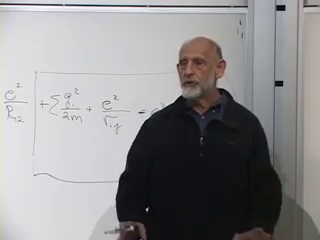
\includegraphics[width=0.72\textwidth]{lecture_01_figure_02.png}
\caption{Hamiltonian phân tử vẫn còn trên bảng khi bài toán trạng thái cơ bản điện tử được đưa ra. Dạng đánh máy trong phương trình~\eqref{eq:molecular-hamiltonian} ghi lại các hạng bị che khuất trong khung hình này.}
\lectureframe{00:16:19}
\end{figure}

\begin{classroomqa}
\audiencequestion{Có phải các xung lượng hạt nhân đơn giản là đang được đặt bằng không không?\lecturetimestamp{00:15:39}}
\lecturerresponse{Chỉ là tạm thời. Trong gần đúng bậc đầu, các hạt nhân được coi như bị ghim chặt vì chúng chuyển động chậm hơn electron rất nhiều. Xung lượng của chúng sẽ được khôi phục khi ta giải bài toán hạt nhân hiệu dụng, nên gần đúng này không vi phạm nguyên lý bất định.}
\end{classroomqa}

Năng lượng trạng thái cơ bản điện tử giờ đây đóng góp vào thế năng mà các hạt nhân cảm nhận:
\begin{equation}
V_{\mathrm{eff}}(R_1,R_2)
=\frac{e^2}{R_{12}}+E_{\mathrm{el}}(R_1,R_2).
\label{eq:molecular-effective-potential}
\end{equation}
Bất biến quay và tịnh tiến, đối với hai nguyên tử cô lập, thu gọn nó thành một hàm của khoảng cách giữa chúng \(R_{12}\). Ở khoảng cách rất ngắn, lực đẩy Coulomb hạt nhân chiếm ưu thế. Ở khoảng cách rất lớn thì hầu như không có tương tác. Giữa hai giới hạn đó, đám mây electron có thể tạo ra một vùng hút và một cực tiểu. Khi ấy, hàm sóng hạt nhân tập trung gần cực tiểu đó và mô tả một phân tử liên kết.

Hãy chú ý đến thứ tự các bước. Ta đã không đoán một lực hút thực nghiệm rồi bỏ các electron đi. Trước hết ta giải bài toán lượng tử của chúng trong nền hạt nhân cố định. Chỉ sau đó ta mới xóa các tọa độ tường minh của chúng và giữ lại trị riêng thu được. Vật lý khoảng cách ngắn vẫn còn trong hình dạng, độ sâu và độ cong của \(V_{\mathrm{eff}}\). Vị trí cực tiểu của nó đặt ra khoảng cách cân bằng, độ cong của nó chi phối các dao động nhỏ, và dạng tiệm cận của nó quyết định liệu có tồn tại trạng thái liên kết hay không. Một hàm hiệu dụng duy nhất mang toàn bộ thông tin điện tử đó vào bài toán chậm hơn.

Như vậy, một Hamiltonian nhiều electron phức tạp đã trở thành một Hamiltonian hạt nhân hai vật với một thế năng mới. Ta đã loại bỏ các bậc tự do nhanh, nhưng vẫn giữ lại trọn vẹn hiệu ứng năng lượng thấp của chúng. Thế năng đã được tái chuẩn hóa. Lập luận Born--Oppenheimer quen thuộc này thường không được giới thiệu dưới tên đó, nhưng nó chứa chính xác ý tưởng ta cần:
\begin{equation}
\begin{gathered}
\text{fast microscopic dynamics}\\
\Downarrow\\
\text{effective parameters for slow dynamics}
\end{gathered}
\end{equation}

\section{Đơn vị tự nhiên và thứ nguyên của một trường}

Trong lý thuyết trường lượng tử, các mode cần bị loại bỏ có thể được mô tả tương đương như các mode khoảng cách ngắn, bước sóng ngắn, tần số cao hoặc năng lượng cao. Trước khi vẽ giản đồ, ta hãy thống nhất cách theo dõi thứ nguyên.

Cơ học thông thường dùng các đơn vị độc lập cho độ dài, thời gian và khối lượng. Trong vật lý hạt, ta đặt
\begin{equation}
\hbar=c=1.
\end{equation}
Khi đó năng lượng và khối lượng là tương đương theo \(E=mc^2\), độ dài và thời gian là tương đương vì \(c=1\), và \(\hbar=1\) khiến xung lượng là nghịch đảo của độ dài. Chỉ còn lại một thứ nguyên:
\begin{equation}
[M]=[E]=[p]=L^{-1},
\qquad
[x]=[t]=L.
\label{eq:natural-units}
\end{equation}

Điều này không xóa bỏ thứ nguyên. Nó chọn các hệ số chuyển đổi sao cho một khoảng thời gian có thể được biểu diễn như một độ dài và một khối lượng như nghịch đảo của độ dài. Một khi đã chỉ định một đơn vị, mọi đơn vị khác đều suy ra theo. Vì thế, một ngưỡng cắt có thể được mô tả hoặc là một khoảng cách ngắn \(\delta\) hoặc là một năng lượng cao \(\Lambda=1/\delta\): đó là cùng một thang đo được diễn đạt bằng hai ngôn ngữ.

Xét một trường vô hướng thực \(\phi\), với mật độ Lagrangian được chuẩn hóa theo dạng sơ lược
\begin{equation}
\mathcal L=(\partial_\mu\phi)(\partial^\mu\phi)-V(\phi),
\qquad
S=\int d^4x\,\mathcal L.
\label{eq:scalar-action}
\end{equation}

\begin{figure}[htbp]
\centering
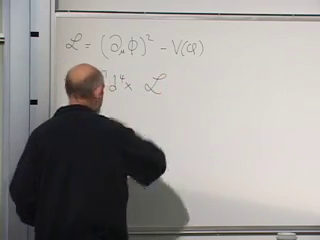
\includegraphics[width=0.78\textwidth]{lecture_01_figure_03.png}
\caption{Mật độ Lagrangian vô hướng cục bộ và tích phân không-thời gian của nó tạo thành tác dụng.}
\lectureframe{00:26:08}
\end{figure}

Mật độ Lagrangian là cục bộ: nó mô tả một điểm không-thời gian. Các phương trình trường cổ điển thu được bằng cách làm cho tác dụng dừng. Trong lý thuyết lượng tử, cũng chính tác dụng ấy xuất hiện trong pha của tích phân đường \(\exp(iS)\). Dù nhìn theo cách nào, thứ nguyên của \(S\) cũng là yếu tố quyết định. Khi khôi phục \(\hbar\), pha là \(\exp(iS/\hbar)\); sau khi đặt \(\hbar=1\), bản thân \(S\) phải là vô thứ nguyên.

\begin{classroomqa}
\audiencequestion{Tác dụng có đơn vị là \(\hbar\) không?\lecturetimestamp{00:26:13}}
\lecturerresponse{Có. Vì \(\hbar\) đã được đặt bằng một, nên tác dụng là vô thứ nguyên trong hệ đơn vị này. Phần tử đo bốn chiều có thứ nguyên \(L^4\), nên mật độ Lagrangian phải có thứ nguyên \(L^{-4}\).}
\end{classroomqa}

Bây giờ hạng động năng xác định thứ nguyên của trường:
\begin{align}
[S]&=1, & [\mathcal L]&=L^{-4},\\
[\partial_\mu]&=L^{-1}, &
[(\partial\phi)^2]&=L^{-2}[\phi]^2=L^{-4},\nonumber\\
&& [\phi]&=L^{-1}.
\label{eq:scalar-dimension}
\end{align}
Phép tính nhỏ này sẽ quyết định bậc tử ngoại của mọi giản đồ tiếp theo.

Khai triển thế năng thành
\begin{equation}
V(\phi)=\frac{m^2}{2}\phi^2+g\phi^3+\lambda\phi^4+\cdots.
\label{eq:scalar-potential}
\end{equation}
Mỗi hạng phải có thứ nguyên \(L^{-4}\). Vì \([\phi^n]=L^{-n}\),
\begin{equation}
[m^2]=L^{-2},
\qquad
[g]=L^{-1},
\qquad
[\lambda]=1.
\label{eq:coupling-dimensions}
\end{equation}
Hằng ghép bậc bốn là vô thứ nguyên. Những hằng ghép như vậy đặc biệt quan trọng trong tái chuẩn hóa vì sự phụ thuộc theo thang đo của chúng không thể đọc ra từ một lũy thừa đơn giản của độ dài.

\begin{classroomqa}
\audiencequestion{\(g\) có đơn vị của khối lượng không?\lecturetimestamp{00:29:52}}
\lecturerresponse{Có. Thừa số \(\phi^3\) có thứ nguyên \(L^{-3}\), còn mật độ thế năng phải có thứ nguyên \(L^{-4}\). Do đó \([g]=L^{-1}\), tức là khối lượng trong đơn vị tự nhiên.}
\end{classroomqa}

\section{Các đỉnh và hàm truyền ở khoảng cách ngắn}

Các quy tắc Feynman được xây dựng từ các đỉnh và các hàm truyền. Hạng \(g\phi^3\) cho một đỉnh ba đường mang một hệ số tỉ lệ với \(g\); \(\lambda\phi^4\) cho một đỉnh bốn đường mang một hệ số tỉ lệ với \(\lambda\). Hạng bậc hai cho một phép chèn hai điểm cục bộ. Có thể hình dung nó như một hạt đi vào, bị hấp thụ, rồi được phát ra trở lại, với hệ số tỉ lệ với \(m^2/2\). Các chuẩn hóa số, dấu, các thừa số của \(i\) và các hệ số đối xứng đều cố ý được lược bỏ vì bài giảng đang rút ra sự phụ thuộc theo thang đo chứ không tính một tiết diện tán xạ.

Các hình vẽ này có một cách hiểu theo thao tác. Một đỉnh ba điểm có thể hấp thụ hai lượng tử và phát ra một lượng tử, hoặc biểu diễn bất kỳ cách gán nào cho ba đường của nó liên hệ với đó qua phép crossing. Một đỉnh bốn điểm có thể mô tả hai hạt đi vào và hai hạt đi ra. Dấu chữ thập bậc hai vẫn là một đỉnh hai đường hoàn toàn hợp lệ dù thông thường nó được gộp vào hàm truyền tự do. Ta vẽ nó ra vì mọi quá trình hai điểm chưa được phân giải rồi sẽ sớm được nhận ra bằng cách so sánh với nó.

Một hàm truyền nối hai điểm không-thời gian. Đường của nó không phải là khẳng định rằng một hạt lượng tử đã đi theo một quỹ đạo cổ điển thẳng. Nó biểu diễn biên độ để tạo ra một kích thích trường tại \(x\) và loại bỏ hoặc dò được nó tại \(y\):
\begin{equation}
\Delta(x-y)=\langle0|\phi(y)\phi(x)|0\rangle.
\label{eq:position-propagator}
\end{equation}
Hãy đọc biểu thức từ bên phải. Tác dụng lên chân không bằng \(\phi(x)\) tạo ra một thành phần một hạt tại \(x\). Tác dụng \(\phi(y)\) lên bra loại bỏ thành phần tại \(y\). Phần tử ma trận chân không của chúng là biên độ chồng lấp giữa sự tạo ra ở điểm thứ nhất và sự dò được ở điểm thứ hai. Các ký hiệu \(x\) và \(y\) chỉ toàn bộ các bốn-vectơ, không chỉ đơn thuần là hai tọa độ Descartes.

Các trạng thái không mang thứ nguyên vật lý, còn mỗi trường đóng góp \(L^{-1}\). Vì vậy
\begin{equation}
[\Delta]=L^{-2}.
\end{equation}
Đối với một trường không khối lượng, không có thang độ dài nội tại nào, nên phân tích thứ nguyên buộc hành vi ở khoảng cách ngắn phải là
\begin{equation}
\Delta(x-y)\sim\frac{1}{(x-y)^2}.
\label{eq:massless-propagator}
\end{equation}
Mẫu số là bình phương độ tách bất biến Lorentz, kèm theo quy định thông thường cần dùng tại các điểm kỳ dị của nó.\editorialnote{Để đếm lũy thừa, thuận tiện là thực hiện phép quay Wick sang độ tách Euclid, khi đó độ lớn rõ ràng tỉ lệ với \(1/|x-y|^2\). Điều này không làm thay đổi các lũy thừa tử ngoại được dùng bên dưới.}

Khi \(y\) tiến tới \(x\), hàm truyền phân kỳ. Điểm kỳ dị này của sự truyền trên một độ tách tiêu biến là nguồn từ đó các phân kỳ tử ngoại trong những giản đồ phức tạp hơn được xây dựng nên.

\section{Khối lượng của trường vô hướng được tái chuẩn hóa như thế nào}

Đối với một trường vô hướng, tham số động lực học là \(m^2\), như hệ thức tán sắc tương đối tính đã gợi ý:
\begin{equation}
E=\sqrt{\mathbf p^2+m^2}.
\end{equation}
Gọi \(\delta\) là khoảng cách ngắn nhất mà mô tả hiệu dụng của ta phân giải được. Ta sẽ không phân biệt các quá trình có các đỉnh cách nhau ít hơn \(\delta\). Bất kỳ quá trình không phân giải được nào như vậy với một vô hướng đi vào và một vô hướng đi ra đều có cùng dạng hai điểm quan sát được như một phép chèn khối lượng và vì thế phải đóng góp vào khối lượng hiệu dụng.

Hãy xem máy gia tốc như một kính hiển vi. Nếu độ phân giải tốt nhất của nó là \(\delta\), thì một sự hấp thụ tại một điểm rồi tiếp theo là một sự phát ra ở một khoảng cách nhỏ hơn rất nhiều so với \(\delta\) sẽ không thể phân biệt được với một biến cố thực sự cục bộ. Ta cố ý làm mờ đỉnh trên thang đó. Tái chuẩn hóa là quy tắc chuyển tất cả những khả năng dưới độ phân giải như vậy vào hệ số của toán tử cục bộ tương ứng.

\subsection{Hiệu chỉnh bậc bốn thứ nhất}

Bắt đầu với một đỉnh \(\phi^4\) đơn lẻ. Hai chân là của hạt ngoài; hai chân kia nối lại thành một vòng ngắn được phát ra rồi hấp thụ lại gần như tại cùng một điểm. Làm mờ hàm truyền trùng điểm trên khoảng cách ngưỡng cắt cho
\begin{equation}
\Delta(0)\ \longrightarrow\ \Delta(\delta)\sim\frac{1}{\delta^2},
\end{equation}
và do đó
\begin{equation}
\delta m^2_{(1)}\sim\frac{\lambda}{\delta^2}.
\label{eq:one-loop-scalar-mass}
\end{equation}
Nếu \(m_0^2\) ký hiệu tham số đầu vào hay tham số trần, thì hệ số hai điểm ở độ phân giải thấp có dạng phác thảo
\begin{equation}
\frac{m_{\mathrm{eff}}^2}{2}
\sim
\frac{m_0^2}{2}
+c_1\frac{\lambda}{\delta^2},
\label{eq:first-renormalized-mass}
\end{equation}
trong đó \(c_1\) chứa các hệ số số học và phụ thuộc quy ước đã bị bỏ qua. Khối lượng đo được trong phòng thí nghiệm, trong những thí nghiệm không phân giải các khoảng cách nhỏ hơn \(\delta\), là đại lượng đã tái chuẩn hóa này, chứ không phải riêng \(m_0\).

Vì thế có hai cách không thể phân biệt được để biến cố hai điểm quan sát được xảy ra. Đỉnh bậc hai ban đầu có thể hấp thụ rồi phát lại hạt, hoặc tương tác bậc bốn có thể làm vậy trong khi thoáng chốc phát ra rồi hấp thụ lại một vô hướng ảo. Cơ học lượng tử cộng các biên độ. Một khi vòng nằm dưới thang phân giải, lịch sử riêng của nó biến mất khỏi mô tả hiệu dụng, nhưng đóng góp của nó vào hệ số đo được thì không.

\subsection{Hiệu chỉnh bậc bốn tiếp theo}

Bây giờ hãy nối hai đỉnh bậc bốn sao cho một hạt ngoài đi vào tại \(x\), một hạt đi ra từ \(x+\Delta\), và ba hàm truyền nội nối hai đỉnh. Có hai lũy thừa của \(\lambda\), còn các hàm truyền cho \(\Delta^{-6}\). Các biên độ lượng tử phải được cộng trên mọi vị trí không phân giải được mà tại đó hạt đi ra có thể xuất hiện, nên bốn-vectơ tương đối được lấy tích phân:
\begin{equation}
\delta m^2_{(2)}
\sim
\lambda^2
\int_{|\Delta|\gtrsim\delta}
d^4\Delta\,\frac{1}{|\Delta|^6}.
\label{eq:two-loop-power-count}
\end{equation}

\begin{classroomqa}
\audiencequestion{Dấu nhỏ ở đỉnh có nghĩa là ở đó chỉ có ba hạt thôi sao?\lecturetimestamp{00:46:35}}
\lecturerresponse{Không. Ta vẫn đang dùng tương tác bậc bốn. Bốn đường gặp nhau tại mỗi đỉnh; trong giản đồ hai điểm này một đường là ngoài và ba đường chạy giữa hai đỉnh. Đỉnh thứ hai lại có bốn đường đi vào nó.}
\end{classroomqa}

Phần tử đo đóng góp bốn lũy thừa của độ dài và ba hàm truyền đóng góp âm sáu. Vì ngưỡng cắt tử ngoại là thang duy nhất trong ước lượng này,
\begin{equation}
\int_{|\Delta|\gtrsim\delta}
\frac{d^4\Delta}{|\Delta|^6}
\sim\frac{1}{\delta^2},
\qquad
\delta m^2_{(2)}
\sim\frac{\lambda^2}{\delta^2}.
\label{eq:two-loop-scalar-mass}
\end{equation}
Ở đây \(\Delta^\mu\) là một biến tích phân bốn thành phần; ta tích phân theo thành phần thời gian và ba thành phần không gian của nó. Chữ thường \(\delta\) là ngưỡng cắt cố định. Ban đầu bài giảng dùng cùng một tên khi phát âm cho cả hai rồi về sau sửa lại ký hiệu.

Có thể thấy cùng kết quả bằng cách viết phần tử đo bốn chiều theo biến bán kính. Bỏ qua một hằng số góc,
\begin{equation}
\int_{\delta}\frac{d^4\Delta}{|\Delta|^6}
\sim
\int_{\delta}\frac{R^3\,dR}{R^6}
=\int_{\delta}\frac{dR}{R^3}
\sim\frac{1}{\delta^2}.
\end{equation}
Đó là lý do vì sao cận trên ở khoảng cách lớn không quan trọng đối với ước lượng tử ngoại: tích phân bị chi phối bởi đầu mút dưới của nó.

Các giản đồ bậc cao hơn lặp lại khuôn mẫu ấy. Một giản đồ với nhiều đỉnh bậc bốn hơn sẽ thêm một lũy thừa cao hơn của \(\lambda\), nhưng phân tích thứ nguyên vẫn cho phép một đóng góp khối lượng phân kỳ bậc hai:
\begin{equation}
\begin{aligned}
m_{\mathrm{eff}}^2
={}&m_0^2
+\frac{1}{\delta^2}
\left(c_1\lambda+c_2\lambda^2+c_3\lambda^3+\cdots\right)\\
&+\text{weaker terms}.
\end{aligned}
\label{eq:scalar-mass-series}
\end{equation}

\subsection{Tương tác bậc ba và một lôgarit}

Hai đỉnh bậc ba chứa hai hàm truyền giữa các điểm gần nhau. Đóng góp của chúng tỷ lệ như
\begin{equation}
\delta m_g^2
\sim
g^2\int_{|\Delta|\gtrsim\delta}
\frac{d^4\Delta}{|\Delta|^4}.
\label{eq:cubic-loop}
\end{equation}
Bây giờ phần tử đo và mẫu số mang các lũy thừa bằng nhau. Sự phụ thuộc còn lại là theo lôgarit chứ không phải theo lũy thừa:
\begin{equation}
\delta m_g^2
\sim
c_g g^2\log\!\left(\frac{1}{\mu\delta}\right).
\label{eq:cubic-log}
\end{equation}
Thang chuẩn \(\mu\) làm cho lôgarit trở thành không thứ nguyên. Đây là phiên bản có đủ thứ nguyên của biểu thức phác thảo trong bài giảng \(g^2\log\delta\). Một lôgarit biến thiên chậm hơn rất nhiều so với bất kỳ lũy thừa nghịch đảo nào, nên \(1/\delta^2\) trội hơn khi ngưỡng cắt trở nên nhỏ.

Một lần nữa, dạng theo bán kính làm cho sự khác biệt hiện ra rõ ràng:
\begin{equation}
\int_{\delta}^{R_{\mathrm{IR}}}
\frac{d^4\Delta}{|\Delta|^4}
\sim
\int_{\delta}^{R_{\mathrm{IR}}}\frac{R^3\,dR}{R^4}
=\log\!\left(\frac{R_{\mathrm{IR}}}{\delta}\right).
\end{equation}
Các lũy thừa bằng nhau ở phần tử đo và mẫu số sinh ra một lôgarit. Nhiều lũy thừa hơn ở mẫu số sinh ra một lũy thừa nghịch đảo của ngưỡng cắt. Bài giảng không yêu cầu ta tính các hệ số góc; nó dạy ta nhận ra đáp án tử ngoại ngay khi nhìn thấy.

\begin{classroomqa}
\audiencequestion{Lôgarit được lấy theo cơ số nào?\lecturetimestamp{00:57:42}}
\lecturerresponse{Hãy dùng lôgarit tự nhiên. Việc đổi cơ số chỉ nhân nó với một hằng số số học, và hằng số đó được hấp thụ vào hệ số mà các thừa số \(2\), \(\pi\) và các hệ số đối xứng của nó chưa được tính ở đây.}
\end{classroomqa}

\begin{classroomqa}
\audiencequestion{Làm sao có thể lấy lôgarit của một độ dài, và thứ nguyên của hiệu chỉnh khối lượng đến từ đâu?\lecturetimestamp{00:58:32}}
\lecturerresponse{Lôgarit luôn so sánh hai thang; nói cho đúng, đó là lôgarit của một tỉ số không thứ nguyên như \(1/(\mu\delta)\). Hằng ghép \(g\) có một lũy thừa khối lượng, nên \(g^2\) đã có đúng thứ nguyên bình phương khối lượng cần cho hiệu chỉnh.}
\end{classroomqa}

\begin{classroomqa}
\audiencequestion{Một giản đồ Feynman cho một biên độ. Bình phương độ lớn của nó có phải là một xác suất không?\lecturetimestamp{00:59:41}}
\lecturerresponse{Có, khi biên độ được đặt vào một phép tính chuyển tiếp vật lý với các thừa số trạng thái và không gian pha cần thiết. Ở đây vai trò trực tiếp hơn của nó lại khác: một biên độ hai điểm không phân giải được có cùng dạng cục bộ như hạng khối lượng và vì thế làm dịch chuyển tham số khối lượng hiệu dụng.}
\end{classroomqa}

\section{Mọi tham số đều trở thành hiệu dụng}

Họ vô hạn các giản đồ khối lượng không biến mất chỉ vì \(\lambda\) nhỏ. Lý thuyết nhiễu loạn sắp xếp chúng theo các lũy thừa của hằng ghép, nên các hạng kế tiếp có thể nhỏ dần, nhưng vẫn có vô hạn hạng. Việc loại bỏ khoảng cách ngắn ấy cũng tái chuẩn hóa chính các tương tác.

\begin{classroomqa}
\audiencequestion{Ngay cả đối với tái chuẩn hóa khối lượng, chẳng phải cũng có vô hạn giản đồ sao?\lecturetimestamp{01:00:35}}
\lecturerresponse{Đúng là có. Nếu \(\lambda\) đủ nhỏ thì chuỗi nhiễu loạn có thể hữu ích vì các lũy thừa cao hơn bị dập tắt dần. Tuy nhiên, tham số đã tái chuẩn hóa được xác định bởi toàn bộ chuỗi, chứ không chỉ bởi hình vẽ đầu tiên thôi.}
\end{classroomqa}

Về mặt thao tác, một tương tác cục bộ \(\lambda\phi^4\) là một biên độ hai hạt vào, hai hạt ra. Nếu một quá trình bốn điểm phức tạp hơn xảy ra hoàn toàn bên trong một vùng không phân giải được, thì ở độ phân giải thấp nó không thể phân biệt được với đỉnh cục bộ ban đầu. Vì thế các giản đồ như vậy được gộp vào một \(\lambda\) hiệu dụng. Sự phụ thuộc theo thang chủ đạo của chúng trong lý thuyết \(\phi^4\) bốn chiều thường là theo lôgarit. Bài giảng không tính hàm beta đó; nó dùng ví dụ này để phát biểu mệnh đề tổng quát:
\begin{equation}
\begin{gathered}
\text{parameters measured at low energy}\\
\ne\\
\text{parameters entered at the microscopic cutoff}
\end{gathered}
\end{equation}

Ví dụ bốn điểm quan trọng vì nó loại bỏ một khả năng hiểu sai. Tái chuẩn hóa không phải là một phép sửa chữa đặc biệt chỉ áp dụng cho một phân kỳ khối lượng. Mọi toán tử được phép trong Lagrangian đều có thể được tái tạo bởi các giản đồ không phân giải được có cùng các chân ngoài và các đối xứng. Một quá trình hai điểm tái chuẩn hóa một hệ số bậc hai, một quá trình bốn điểm tái chuẩn hóa một hệ số bậc bốn, và các quá trình từ chân không đến chân không sẽ tái chuẩn hóa hạng hằng. Lagrangian năng lượng thấp là sổ cái cô đọng trong đó mọi quá trình khoảng cách ngắn ấy được ghi lại.

\begin{classroomqa}
\audiencequestion{Vì \(\Delta\) có đơn vị độ dài, phải chăng lấy lôgarit của nó là lạ về mặt thứ nguyên? Và trên bảng có đổi lẫn delta viết hoa với viết thường không?\lecturetimestamp{01:01:34}}
\lecturerresponse{Lôgarit thực ra có nghĩa là một tỉ số với một thang khác và vì thế là không thứ nguyên. Đúng, ký hiệu đã bị đổi lẫn trong chốc lát: \(\Delta^\mu\) là biến tích phân, còn \(\delta\) là ngưỡng cắt khoảng cách ở cận dưới còn lại trong đáp án.}
\end{classroomqa}

Đây là đối ứng trong lý thuyết trường của phân tử. Ta đã giải đối với các electron nhanh không nhìn thấy và đưa kết quả của chúng vào một thế. Ở đây ta cộng các quá trình khoảng cách ngắn không nhìn thấy và đưa kết quả của chúng vào các khối lượng, các hằng ghép và mọi hệ số cục bộ được phép khác. Mọi thứ đều bị dịch chuyển.

\begin{classroomqa}
\audiencequestion{Thầy có thể nhắc lại liệu đại lượng đo được có bao gồm các thang nhỏ hơn mức thí nghiệm có thể thấy hay không không?\lecturetimestamp{01:05:13}}
\lecturerresponse{Có. Những thăng giáng riêng lẻ của chúng không được phân giải, nhưng hiệu ứng tổng cộng của chúng thì có mặt. Mọi giản đồ liên quan đến các thang ngắn hơn đều được gộp vào một hệ số hiệu dụng duy nhất mà một thí nghiệm năng lượng thấp gọi, chẳng hạn, là bình phương khối lượng vật lý.}
\end{classroomqa}

\begin{classroomqa}
\audiencequestion{Vậy số hạng đầu vào \(m_0^2\) có phải triệt tiêu các đóng góp khác không?\lecturetimestamp{01:06:00}}
\lecturerresponse{Nếu khối lượng vô hướng đo được nhỏ hơn rất nhiều so với các đóng góp tử ngoại riêng lẻ, thì đúng vậy. Sự triệt tiêu cần thiết ấy chính là bài toán tinh chỉnh mà bây giờ ta chuyển sang.}
\end{classroomqa}

\section{Bài toán phân cấp Higgs}

Hãy hình dung ngưỡng cắt là độ dài Planck, để lý thuyết trường hiệu dụng được yêu cầu tóm lược các thăng giáng từ những thang phòng thí nghiệm xuống tới thang mà hấp dẫn lượng tử buộc phải can thiệp.
Trong các đơn vị của vật lý hạt,
\begin{equation}
\delta\sim M_{\mathrm{Pl}}^{-1}\sim10^{-19}\,\mathrm{GeV}^{-1},
\qquad
\frac{1}{\delta^2}\sim10^{38}\,\mathrm{GeV}^2.
\label{eq:planck-cutoff}
\end{equation}
Việc dùng chính xác thang Planck rút gọn hay không rút gọn không quan trọng đối với phép so sánh khổng lồ này.

Phân cấp về khoảng cách cũng nổi bật không kém. Độ dài Planck nhỏ hơn bán kính proton khoảng 19 bậc độ lớn và nhỏ hơn các khoảng cách được các máy gia tốc đang được bàn đến thăm dò trực tiếp khoảng 16 hoặc 17 bậc. Việc bình phương độ tách ấy chính là điều biến một phân cấp độ dài lớn thành sự triệt tiêu cỡ 34 chữ số trong một tham số bình phương khối lượng vô hướng.

Đối với trường Higgs, một trường vô hướng, thang yếu mong muốn có cỡ vài trăm GeV, chứ không phải \(10^{19}\) GeV. Thế nhưng các hạng trong Phương trình~\eqref{eq:scalar-mass-series} một cách tự nhiên có thể có cỡ thang Planck. Dấu của chúng chưa được theo dõi: một số có thể dương và một số có thể âm, và bình phương khối lượng trần cũng có thể mang một trong hai dấu. Nhưng để còn lại một phần dư ở thang điện yếu, những phần khổng lồ ấy phải triệt tiêu nhau tới khoảng 34 chữ số thập phân. Ban đầu Susskind nói 17 chữ số, rồi tự sửa lại vì phép so sánh là giữa các bình phương khối lượng. Chính tỉ số đã được bình phương mới đo phiên bản tinh chỉnh này.

\begin{classroomqa}
\audiencequestion{\(\lambda\) nhỏ hơn hay lớn hơn 1?\lecturetimestamp{01:09:50}}
\lecturerresponse{Người ta giả định nó nhỏ hơn 1 ở mức vừa phải. Lý thuyết nhiễu loạn sẽ trở nên khó xử lý nếu các lũy thừa kế tiếp tăng lên, và một lý thuyết vô hướng thuần túy cũng không thể được ngoại suy một cách nhất quán với một hằng số liên kết tứ bậc lớn tùy ý. Nhưng \(\lambda\) hoàn toàn không nhỏ đến mức như \(10^{-38}\); bài giảng lấy một con số cỡ phần trăm để định hướng.}
\end{classroomqa}

\begin{classroomqa}
\audiencequestion{Ngay cả khi \(\lambda<1\), chẳng phải vẫn còn nhiều hạng giữ vai trò quan trọng vì mỗi hạng đều mang hệ số cắt lớn sao?\lecturetimestamp{01:10:43}}
\lecturerresponse{Đúng vậy. Các lũy thừa cao hơn rốt cuộc sẽ làm suy giảm chuỗi, nhưng trước khi điều đó thắng thế thì vẫn có thể có một tập hợp lớn các hạng đóng góp. Tất cả chúng, cùng với hạng trần, đều sẽ phải cùng nhau triệt tiêu tinh vi để còn lại đáp án vật lý nhỏ phi thường ấy.}
\end{classroomqa}

Nhắc lại vì sao tham số khối lượng Higgs được biết là ở thang yếu. Theo quy ước của bài giảng, viết thế phá vỡ đối xứng dưới dạng
\begin{equation}
V(\phi)=-\frac{\mu^2}{2}\phi^2+\frac{\lambda}{4}\phi^4.
\label{eq:higgs-potential}
\end{equation}
Hệ số bậc hai âm làm cho gốc tọa độ mất ổn định, còn hạng tứ bậc dương làm ổn định thế. Lấy đạo hàm,
\begin{equation}
\frac{dV}{d\phi}=-\mu^2\phi+\lambda\phi^3
=\phi(-\mu^2+\lambda\phi^2),
\end{equation}
cho ta cực tiểu khác không
\begin{equation}
\phi_{\min}^2=f^2=\frac{\mu^2}{\lambda}.
\label{eq:higgs-minimum}
\end{equation}
Trên bảng viết hạng tứ bậc một cách sơ lược là \(\lambda\phi^4\) nhưng lại viện dẫn phương trình ~\eqref{eq:higgs-minimum}; chèn hệ số quy ước \(1/4\) sẽ làm cho hai dòng ấy nhất quán với nhau mà không thay đổi lập luận.

Dấu của \(-\mu^2\) là quan trọng, nhưng không cứu được tính tự nhiên. Chính độ cong âm tại gốc tọa độ là cái thúc đẩy sự phá vỡ đối xứng tự phát. Tái chuẩn hóa làm dịch chuyển độ cong ấy bởi những phần dương và âm rất lớn. Chân không bị phá vỡ mà ta quan sát được đòi hỏi tổng của chúng không chỉ nhỏ, mà còn phải có đúng giá trị âm nhỏ đặc biệt đặt cực tiểu ở thang yếu.

Khối lượng của các boson \(W\) và \(Z\) xác định \(f\) vào cỡ \(200\,\mathrm{GeV}\) trong cách chuẩn hóa gần đúng được dùng trong bài giảng. Nếu \(\lambda\) không quá lớn cũng không nhỏ đến mức khó tin, thì \(\mu\) phải cùng bậc đại thể như vậy. Vì thế, hệ số quan sát được ở thang yếu là phần dư của những đóng góp mà mỗi cái riêng lẻ có thể lớn hơn nhiều chục bậc độ lớn.

Điều này được gọi là bài toán tinh chỉnh Higgs, bài toán phân cấp, hoặc bài toán phân cấp chuẩn. Phân cấp ở đây là tỉ số khổng lồ giữa thang yếu thông thường và một thang thống nhất hoặc Planck khả dĩ. Một số nhỏ tự nó chưa chắc đã là nghịch lý. Điều gây bất an ở đây là một số nhỏ được ghép từ những phần lớn, có vẻ không liên hệ với nhau, nhưng lại phải triệt tiêu nhau với độ chính xác cực cao. Bài toán này đã được nhận ra vào cuối thập niên 1970 và đầu thập niên 1980, và việc tìm một cơ chế đằng sau sự triệt tiêu ấy đã thúc đẩy siêu đối xứng cùng một số ý tưởng cạnh tranh khác.

Chuỗi nhiễu loạn vô hạn làm cho câu đố sắc nét hơn chứ không loại bỏ nó. Một \(\lambda\) cỡ phần trăm khiến các lũy thừa đủ cao trở nên nhỏ, nhưng có thể xuất hiện nhiều hạng trước khi sự suy giảm ấy thắng thế. Không đủ nếu một vòng tình cờ triệt tiêu khối lượng trần. Thang yếu hiệu dụng phải vẫn ổn định sau khi đã tính cả phần còn lại của các quá trình khoảng cách ngắn. Một quan hệ có tính cấu trúc giữa các hạng mới là lời giải thích; một sự triệt tiêu từng chữ số giữa những phần không liên hệ chỉ là tinh chỉnh.

\section{Vì sao khối lượng fermion ứng xử tốt hơn}

Các hạt khác của Mô hình Chuẩn không đòi hỏi những sự tinh chỉnh độc lập cùng loại. Với một fermion Dirac, hạng khối lượng là
\begin{equation}
\mathcal L_m=-m\bar\psi\psi
=-m\left(\bar\psi_L\psi_R+\bar\psi_R\psi_L\right).
\label{eq:fermion-mass}
\end{equation}
Nó chứa khối lượng, không phải bình phương của khối lượng, và nó nối chirality trái với chirality phải. Vì thế, một phép chèn khối lượng cục bộ biến \(L\) thành \(R\), hoặc \(R\) thành \(L\).

\begin{figure}[htbp]
\centering
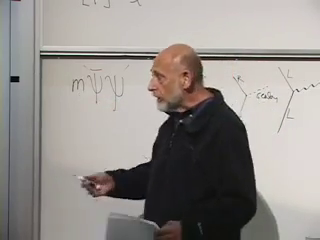
\includegraphics[width=0.76\textwidth]{lecture_01_figure_04.png}
\caption{Hạng khối lượng fermion và các phác họa đường làm đổi chirality trên bảng. Các hình được dựng lại bằng đại số ở dưới vì một phần nét phấn bị che khuất.}
\lectureframe{01:23:36}
\end{figure}

Trong phần trình bày miệng, giảng viên thường nói đến tính thuận tay hoặc helicity. Sự bảo vệ chính xác được phát biểu sáng sủa nhất theo chirality. Đối với một hạt siêu tương đối tính, hình dung theo helicity cung cấp trực giác mà bài giảng nhắm tới, nhưng chirality mới là đại lượng do các trường tay trái và tay phải trong phương trình~\eqref{eq:fermion-mass} mang.

Tương tác chuẩn bảo toàn chirality:
\begin{equation}
L\xrightarrow{\ \gamma\ }L,
\qquad
R\xrightarrow{\ \gamma\ }R.
\label{eq:gauge-preserves-chirality}
\end{equation}
Một tương tác Yukawa với một trường vô hướng nối hai chirality đối nhau:
\begin{equation}
L\xleftrightarrow{\ \phi\ }R.
\label{eq:scalar-flips-chirality}
\end{equation}
Trước hết, giả sử \(m_0=0\). Việc phát xạ rồi tái hấp thụ bất kỳ số photon nào cũng không thể sinh ra khối lượng, vì mọi đỉnh chuẩn đều bảo toàn chirality. Một chuỗi bắt đầu với chirality trái sẽ vẫn là chirality trái. Vì vậy, điện động lực học lượng tử thuần túy cho phép một electron không khối lượng một cách nhất quán: tự năng điện từ của nó không thể tạo ra một khối lượng cộng thêm từ số 0.

Trong hình ảnh đường, hãy bắt đầu với một electron có chirality trái. Ở đỉnh photon thứ nhất nó vẫn có chirality trái; sau khi truyền đi và tái hấp thụ photon nó vẫn có chirality trái. Lặp lại cấu trúc ấy chỉ chèn thêm các đỉnh bảo toàn chirality. Hàm hai điểm ngoài có thể được tái chuẩn hóa, nhưng nó không thể nhận được cấu trúc trái-phải vốn định nghĩa một khối lượng.

Phát xạ vô hướng có làm được điều đó không? Một đỉnh vô hướng biến \(L\) thành \(R\), nhưng một vô hướng đã phát ra thì phải được tái hấp thụ. Vì thế, một đồ thị tự năng hai điểm chứa một số chẵn các đỉnh vô hướng. Lần lật thứ hai đảo ngược lần thứ nhất, nên toàn bộ đồ thị lại bảo toàn chirality ngoài. Dù đồ thị bên trong có trở nên phức tạp đến đâu, phát xạ và tái hấp thụ vẫn ghép cặp các đỉnh và ngăn không cho xuất hiện một hạng cộng thêm từ \(L\) sang \(R\) khi khối lượng ban đầu bằng 0.

Đây là một lập luận chẵn-lẻ về số lần lật. Một đỉnh vô hướng lật chirality một lần; việc khép kín mỗi đường vô hướng nội đòi hỏi một đầu mút thứ hai và vì thế một lần lật thứ hai. Bốn đỉnh vô hướng lật bốn lần, v.v. Một số chẵn đưa fermion trở về chirality ban đầu của nó. Kết luận này không bị giới hạn ở vòng đơn giản nhất được vẽ trên bảng.

Một hiệu chỉnh khối lượng khác không chỉ trở nên khả dĩ sau khi sơ đồ đã chứa sẵn một phép chèn khối lượng. Chẳng hạn, sự phát xạ và tái hấp thụ photon có thể bao quanh một phép chèn \(m_0\bar\psi\psi\). Các đỉnh chuẩn đóng góp hai lũy thừa của điện tích điện, nhưng lần lật chirality duy nhất đóng góp khối lượng ban đầu:
\begin{equation}
\begin{aligned}
m_e
&=m_0+c_1e^2m_0+c_2e^4m_0+\cdots\\
&=m_0\left(1+c_1e^2+c_2e^4+\cdots\right).
\end{aligned}
\label{eq:multiplicative-fermion-mass}
\end{equation}
Nếu \(m_0=0\), kết quả vẫn bằng không. Nếu \(m_0\) nhỏ, thì mọi hiệu chỉnh đều tỉ lệ với số nhỏ ấy. Ta vẫn có thể hỏi vì sao electron lại nhẹ so với một thang cơ bản, nhưng ta không còn phải lấy những số khổng lồ không liên hệ mà trừ vào nhau để thu được nó nữa. Theo nghĩa này, một khối lượng fermion nhỏ là tự nhiên theo nghĩa kỹ thuật.

Phép chèn khối lượng làm cho chuỗi được phép trở nên tường minh. Bắt đầu với \(L\). Phát xạ photon bảo toàn \(L\); phép chèn \(m_0\) biến \(L\) thành \(R\); tái hấp thụ photon bảo toàn \(R\). Khi đó, sơ đồ có chirality ngoài của một hạng khối lượng, nhưng giá trị của nó tất yếu chứa thừa số \(m_0\). Đây là sự tương phản then chốt với phương trình ~\eqref{eq:one-loop-scalar-mass}, ở đó hiệu chỉnh vô hướng vẫn khác không ngay cả khi khối lượng vô hướng ban đầu được đặt bằng không.

Các boson chuẩn có một sự bảo vệ tương tự: đối xứng chuẩn cấm một hạng khối lượng độc lập, nên một boson chuẩn ban đầu không khối lượng sẽ vẫn không khối lượng ở mọi bậc nhiễu loạn. Trong Mô hình Chuẩn, khối lượng của các fermion và các boson chuẩn yếu phát sinh do giá trị kỳ vọng Higgs. Nếu kiểm soát được thang Higgs, thì các khối lượng nhẹ còn lại không cần những lần lặp riêng rẽ của cùng một sự tinh chỉnh thảm khốc ấy.

Điều này xác định câu hỏi mà siêu đối xứng được kỳ vọng sẽ giải quyết: liệu một lý thuyết có thể ngăn không cho vô hướng Higgs nhận một hiệu chỉnh khối lượng cộng thêm khổng lồ hay không? Câu trả lời là có trong những thiết lập siêu đối xứng thích hợp, vì các đóng góp boson và fermion có liên hệ với nhau chứ không độc lập. Cơ chế chi tiết bắt đầu ở bài giảng tiếp theo.

\section{Sự tinh chỉnh khác: năng lượng chân không}

Vẫn còn một bài toán tái chuẩn hóa còn nghiêm trọng hơn, nhưng nó chỉ trở nên quan sát được khi có hấp dẫn. Trong vật lý phi hấp dẫn, việc cộng một hằng số vào mọi năng lượng không làm thay đổi thí nghiệm nào. Chẳng hạn, khối lượng electron không phải là một năng lượng tuyệt đối; nó là năng lượng tăng thêm cần để thêm một electron vào chân không:
\begin{equation}
m_e=E(\text{vacuum}+\text{one electron})-E(\text{vacuum})
\end{equation}
trong hệ nghỉ của electron. Nếu chân không và mọi trạng thái kích thích cùng dịch chuyển, thì các hiệu của chúng vẫn không đổi.

Tuy vậy, các sơ đồ chân không-sang-chân không quả thật làm dịch chuyển năng lượng chân không. Trong lý thuyết \(\lambda\phi^4\), hãy nối bốn chân của một đỉnh tứ bậc thành hai vòng ngắn. Mỗi hàm truyền tại điểm trùng nhau cho \(1/\delta^2\), nên
\begin{equation}
\delta\rho_{\mathrm{vac}}
\sim
c_{\mathrm{vac}}\frac{\lambda}{\delta^4}.
\label{eq:vacuum-energy-divergence}
\end{equation}
Các sơ đồ chân không phức tạp hơn mang những hệ số liên kết và hệ số số học khác nhau, nhưng phân tích thứ nguyên thường vẫn để lại cùng một độ nhạy điểm cắt bậc bốn đối với một mật độ năng lượng.

Chính việc không có các đường ngoài là dấu hiệu nhận ra hiệu chỉnh này. Các đồ thị hai điểm so sánh một trạng thái một hạt với chân không và làm thay đổi khối lượng; các đồ thị bốn điểm làm thay đổi tán xạ; một đồ thị không có hạt đi vào hay đi ra làm thay đổi chính biên độ chân không-sang-chân không. Một đỉnh tứ bậc cho \(\lambda\), và hai vòng ngắn của nó cho \(\delta^{-2}\) mỗi vòng. Khi đó, phân tích thứ nguyên đòi hỏi thang mật độ năng lượng \(\delta^{-4}\).

Không có hấp dẫn, ta có thể chọn mốc 0 cộng tính của năng lượng và hỏi ai quan tâm. Thuyết tương đối rộng tước bỏ tự do ấy: tensor năng lượng-động lượng là nguồn của độ cong không-thời gian, nên một năng lượng chân không đồng đều làm cho không gian trống hấp dẫn. Nó xuất hiện như một hằng số vũ trụ và được liên hệ về mặt quan sát với năng lượng tối. Khi đó, một năng lượng chân không đo được rất nhỏ phải còn lại sau những đóng góp có dạng \(\delta^{-4}\).

Đó là lý do vì sao câu hỏi thay đổi khi đưa hấp dẫn vào. Trong cơ học lượng tử thông thường, dịch mọi mức lên cùng một hằng số không làm động đến bất kỳ tần số chuyển mức nào. Trong hấp dẫn, hằng số ấy không trơ: tensor năng lượng-động lượng của chân không tỉ lệ với metric và làm cong không-thời gian. Điều từng là một mốc 0 năng lượng tùy ý nay trở thành một nguồn trong phương trình Einstein.

Vì vậy có ít nhất hai câu đố về tính tự nhiên ở mức cực đoan. Bài giảng nêu xấp xỉ 123 chữ số thập phân cho mức tinh chỉnh của năng lượng chân không và khoảng 30--35 cho mức tinh chỉnh của khối lượng Higgs. Số lượng chính xác phụ thuộc vào thang tử ngoại và các quy ước, nhưng sự tương phản thì không có gì phải nghi ngờ. Siêu đối xứng là một lời đáp tiềm năng cho bài toán Higgs được bàn ở đây; một khi siêu đối xứng bị phá vỡ, tự thân nó không giải thích được hằng số vũ trụ học quan sát được.\editorialnote{Đây cũng là lý do vì sao một sự triệt tiêu boson--fermion siêu đối xứng chính xác không phải là một lời giải hiện tượng học cho năng lượng chân không quan sát được: siêu đối xứng phải bị phá vỡ trong thế giới của chúng ta.}

\section{Các câu hỏi cuối buổi học}

\begin{classroomqa}
\audiencequestion{Hiệu chỉnh Higgs phụ thuộc vào điểm cắt \(\delta\), nhưng điểm cắt ấy có vẻ tùy ý. Nó có thể là độ dài Planck, gấp 10 lần độ dài Planck, hay một thứ khác không? Điều đó có làm cho sự tinh chỉnh trở nên tùy ý không?\lecturetimestamp{01:33:50}}
\lecturerresponse{Đóng góp số học phụ thuộc vào thang ngắn nhất mà lý thuyết hiệu dụng còn được tin cậy. Sự phụ thuộc ấy là cách hạch toán vật lý, không phải một lối thoát. Các mode đến bất kỳ thang nào mà Mô hình Chuẩn vẫn còn có nghĩa đều là những mode mà hiệu ứng của chúng phải được tính vào. Chọn \(\delta\) tại khoảng cách nơi người ta kỳ vọng có vật lý mới---có thể là thang Planck, có thể là một thang thống nhất gần \(10^{16}\,\mathrm{GeV}\). Đóng góp tích lũy xuống đến thang ấy đã là một cận dưới cho vấn đề rồi. Mở rộng cùng lý thuyết ấy xuống những khoảng cách còn ngắn hơn chỉ làm cho độ nhạy bậc hai lớn hơn. Ta có nghĩa vụ phải giải thích điều gì triệt tiêu đóng góp từ mọi thang giữa phòng thí nghiệm và biên tử ngoại ấy.}
\end{classroomqa}

\begin{classroomqa}
\audiencequestion{Điều gì định nghĩa một hạt vô hướng, và ví dụ là gì?\lecturetimestamp{01:37:26}}
\lecturerresponse{Ví dụ được nhắm đến là Higgs. Một trường vô hướng không biến đổi thành các thành phần khác nhau dưới một phép quay không gian; tương đương, các lượng tử hạt của nó có spin 0. Photon được mô tả bởi một trường vectơ, còn trường hấp dẫn bởi một tenxơ. Vào thời điểm của bài giảng 2010 này, vẫn chưa phát hiện được hạt sơ cấp spin 0 nào.\editorialnote{Boson Higgs được phát hiện tại CERN vào 2012 và các tính chất đo được của nó phù hợp với spin 0.}}
\end{classroomqa}

\begin{classroomqa}
\audiencequestion{Hạt \(Z\) cũng là một boson chuẩn phải không?\lecturetimestamp{01:38:31}}
\lecturerresponse{Có. \(Z\), \(W^+\) và \(W^-\) là các boson chuẩn spin 1; photon cũng vậy. Các phương trình trường và các tương tác của chúng là những khái quát hóa không Abel hoặc điện yếu của mô tả chuẩn kiểu Maxwell.}
\end{classroomqa}

\begin{classroomqa}
\audiencequestion{Tại sao đóng góp của trạng thái cơ bản boson lại không triệt tiêu đóng góp của trạng thái cơ bản fermion trong năng lượng chân không?\lecturetimestamp{01:39:10}}
\lecturerresponse{Các vòng fermion và các vòng boson tương ứng quả thật có thể xuất hiện với dấu đối nhau. Tuy nhiên, sự triệt tiêu không tự động xảy ra: khối lượng, số bội và các hằng số ghép của hạt phải khớp nhau. Chỉ một sai lệch nhỏ cũng để lại một phần dư lớn nhạy với ngưỡng cắt, và các họ giản đồ vô hạn phải khớp nhau theo từng bậc. Siêu đối xứng chính xác áp đặt chính những quan hệ boson--fermion như vậy. Thành phần hạt không siêu đối xứng nói chung thì không như vậy, và siêu đối xứng bị phá vỡ để lại một bài toán năng lượng chân không còn dư.}
\end{classroomqa}

\section{Toàn cảnh}

Lộ trình của bài giảng được sắp đặt có chủ ý. Trước hết, một phép tính phân tử cho thấy rằng việc loại bỏ các biến nhanh không phải là bỏ qua chúng, cũng không phải là phép màu: năng lượng trạng thái cơ bản của chúng trở thành một thế năng đối với các biến chậm. Lý thuyết trường lượng tử lặp lại thao tác đó trên các thang bước sóng. Phân tích thứ nguyên sau đó cho thấy những tham số hiệu dụng nào nhạy với ngưỡng cắt. Khối lượng của các hạt vô hướng nhận các số hạng cộng thêm tỉ lệ với \(\delta^{-2}\); vì vậy, một thang Higgs nhỏ có vẻ mong manh một cách không tự nhiên. Khối lượng fermion được tái chuẩn hóa theo kiểu nhân vì tính tay bảo vệ giới hạn khối lượng bằng không, và đối xứng chuẩn cũng bảo vệ tương tự các boson chuẩn không khối lượng. Năng lượng chân không còn nhạy hơn nữa, có tỉ lệ như \(\delta^{-4}\), và hấp dẫn khiến giá trị tuyệt đối của nó có thể quan sát được.

Siêu đối xứng được đưa vào chính tại điểm này, không phải như một thứ toán học mới mang tính trang trí mà như một nỗ lực làm cho sector vô hướng ứng xử giống các sector được bảo vệ hơn. Nhiệm vụ tiếp theo là hiểu xem đối xứng nào có thể liên hệ boson với fermion đủ chặt chẽ để sắp đặt các sự triệt tiêu đó.
